\documentclass[11pt,a4paper]{article}
\usepackage[margin=1in]{geometry}
\usepackage{amsmath,amssymb}
\usepackage{booktabs}
\usepackage{tabularx}
\usepackage{array}
\usepackage{graphicx}
\usepackage{float}
\usepackage[hidelinks]{hyperref}
\usepackage{enumitem}
\usepackage{xcolor}
\usepackage{pgfplots}
\pgfplotsset{compat=1.18}
\renewcommand{\arraystretch}{1.15}

\title{Comprehensive Status Report\\
3-Class ADNI Brain Graph Classification Pipeline\\
{\large (Phase-1 and Phase-2 Stabilization Focus)}}
\author{Internal Research Progress Note}
\date{March 19, 2026}

\begin{document}
\maketitle

\section{Purpose of This Document}
This report records what changed in the experiment pipeline, why those changes were made, what we observed in runs, and how current results compare with standard baselines and publication-level targets.

\section{Project Context and Goal}
\textbf{Task:} classify each subject graph into CN, AD, or MCI.

\textbf{Challenge:} severe class imbalance and synthetic data reliability. AD is a minority class, so augmentation is needed, but only high-quality synthetic graphs should be retained.

\textbf{Current cycle objective:} stabilize phase-1 and phase-2 first, then evaluate downstream behavior in end-to-end runs.

\section{Pipeline Overview (Phases 1--5)}
\subsection{Phase 1: Generative Training}
\begin{itemize}[leftmargin=1.2em]
    \item VAE learns compressed latent representation of brain graphs.
    \item Latent diffusion learns iterative denoising from noise to plausible graph latents.
    \item Latent teacher learns class structure used later for guided generation.
\end{itemize}

\subsection{Phase 2: Guided Synthetic Generation}
\begin{itemize}[leftmargin=1.2em]
    \item Start from latent noise.
    \item Reverse diffusion denoises with class guidance toward AD/MCI.
    \item Decode latent outputs into synthetic adjacency matrices.
\end{itemize}

\subsection{Phase 3: Synthetic Filtering}
Correlation-based realism/uniqueness filtering with thresholds $\tau_{min},\tau_{max}$.

\subsection{Phase 4: Contrastive Pretraining}
Representation pretraining stage; held mostly fixed in this cycle to isolate phase-1/2 effects.

\subsection{Phase 5: Fine-tuning and Evaluation}
Final supervised classifier training with real + selected synthetic data, evaluated on held-out real test data.

\section{Quality Assessments Added and Why}
\subsection{Phase-1 assessments}
\begin{itemize}[leftmargin=1.2em]
    \item Teacher macro-F1 and class-wise recall.
    \item Confusion behavior and collapse detection.
    \item Run/checkpoint stability checks.
\end{itemize}
\textbf{Reason:} phase-1 teacher quality strongly controls phase-2 generation quality.

\subsection{Phase-2 assessments}
\begin{itemize}[leftmargin=1.2em]
    \item Teacher confidence for target class.
    \item Duplicate risk (vs real and intra-synthetic).
    \item Spectral plausibility (top-k eigen-spectrum distance).
    \item Guidance trajectory monotonicity during reverse diffusion.
    \item Graph topology and edge-distribution plausibility.
\end{itemize}
\textbf{Reason:} these checks jointly measure validity, novelty, plausibility, and generation dynamics.

\subsection{Critical upgrade in this cycle: enforceable gates}
Previously, checks were mostly diagnostic. Added policy controls:
\begin{itemize}[leftmargin=1.2em]
    \item \texttt{quality\_enforce\_gates}
    \item \texttt{quality\_min\_keep}
    \item \texttt{quality\_fallback\_keep\_all}
\end{itemize}
This changed phase-2 from ``observe only to ``observe + control retention.

\section{Loss Functions and Mathematical Foundations}
\subsection{Guided reverse diffusion}
\[
\hat{\epsilon}(x_t,t)=\epsilon_\theta(x_t,t)-\sqrt{1-\bar{\alpha}_t}\,w\,\nabla_{x_t}\log p_\phi(y\mid x_t)
\]
where $w$ is guidance scale and $p_\phi(y\mid x_t)$ is teacher confidence.

\subsection{Final classifier objective}
\[
\mathcal{L}_{CE}=-\frac{1}{N}\sum_{i=1}^{N}\sum_{c=1}^{C} y_{i,c}\log \hat{y}_{i,c}
\]
Cross-entropy variants were used (weighted/unweighted), respecting constraints.

\section{Metrics Positioning vs Baseline, SOTA, and Target}
\begin{table}[H]
\centering
\scriptsize
\begin{tabular}{@{}p{3.2cm}ccccc p{4.0cm}@{}}
\toprule
Reference & Accuracy & Macro-F1 & AUC-OVR & AD Recall & MCI Recall & Notes \\
\midrule
Vanilla StandardGCN baseline (literature) & 0.70--0.72 & ~0.55 & ~0.78 & ~0.45 & ~0.40 & Common baseline operating range \\
BrainGNN (representative published method) & 0.78--0.82 & ~0.65 & ~0.85 & ~0.60 & ~0.55 & Strong peer comparator \\
Recent SOTA range (2024--2025) & 0.88--0.92 & ~0.80 & ~0.94 & ~0.75 & ~0.70 & Top-tier competitive zone \\
Internal publishable target & $>$0.85 & $>$0.75 & $>$0.90 & $>$0.65 & $>$0.60 & Target zone for submission readiness \\
\midrule
Current benchmark (job 13860) & 0.75 & 0.5441 & 0.8092 & 0.15 & 0.49 & Best pre-enforcement reference \\
Best observed this cycle (job 13925) & 0.72 & 0.5496 & 0.7898 & 0.31 & 0.42 & Best Macro-F1 in this cycle \\
\bottomrule
\end{tabular}
\caption{Current standing versus baseline, publication comparators, and internal target metrics.}
\end{table}

\section{Initial and Follow-up Run Observations}
\begin{table}[H]
\centering
\scriptsize
\begin{tabular}{@{}p{1.2cm} p{4.1cm} c c c p{4.6cm}@{}}
\toprule
Job & Setup & Macro-F1 & AUC & AD Recall & Observation \\
\midrule
13860 & Cycle benchmark & 0.5441 & 0.8092 & 0.15 & Reference before current phase-2 enforcement \\
13925 & AD-heavy caps (200/100), no class-weight & \textbf{0.5496} & 0.7898 & 0.31 & Best Macro-F1 observed in this cycle \\
13930 & Similar config (repeat) & 0.5451 & 0.7933 & 0.23 & Confirms headroom; variance remains \\
13959 & E2E baseline (no gate enforcement) & 0.4366 & 0.7873 & 0.00 & AD collapsed \\
13960 & E2E with gate enforcement & 0.3776 & 0.7859 & 0.23 & MCI collapsed due over-pruning \\
\bottomrule
\end{tabular}
\caption{Representative run outcomes used for phase-2 decision making.}
\end{table}

\textbf{Interpretation:}
\begin{itemize}[leftmargin=1.2em]
    \item Higher Macro-F1 is achievable in selected settings, so improvement potential is real.
    \item Current enforced-gate thresholds over-prune in some E2E settings.
    \item Phase-2 changes are valid infrastructure but require calibration with later phases.
\end{itemize}

\section{Validation of New Phase-2 Logic}
Validation run job 13953 confirmed policy behavior:
\begin{itemize}[leftmargin=1.2em]
    \item AD retained 21/120 (below \texttt{min\_keep=30}); fallback preserved AD set.
    \item MCI retained 48/120 (above min-keep); reduced set was saved.
\end{itemize}

\section{Architecture and Flow Figures}
\begin{figure}[H]
\centering
\includegraphics[width=0.95\textwidth]{fig_pipeline_overview.png}
\caption{High-level 3-class pipeline overview.}
\end{figure}

\begin{figure}[H]
\centering
\includegraphics[width=0.92\textwidth]{figure_2.png}
\caption{Phase-2 quality-gate mechanism and retention policy (selected figure).}
\end{figure}

\begin{figure}[H]
\centering
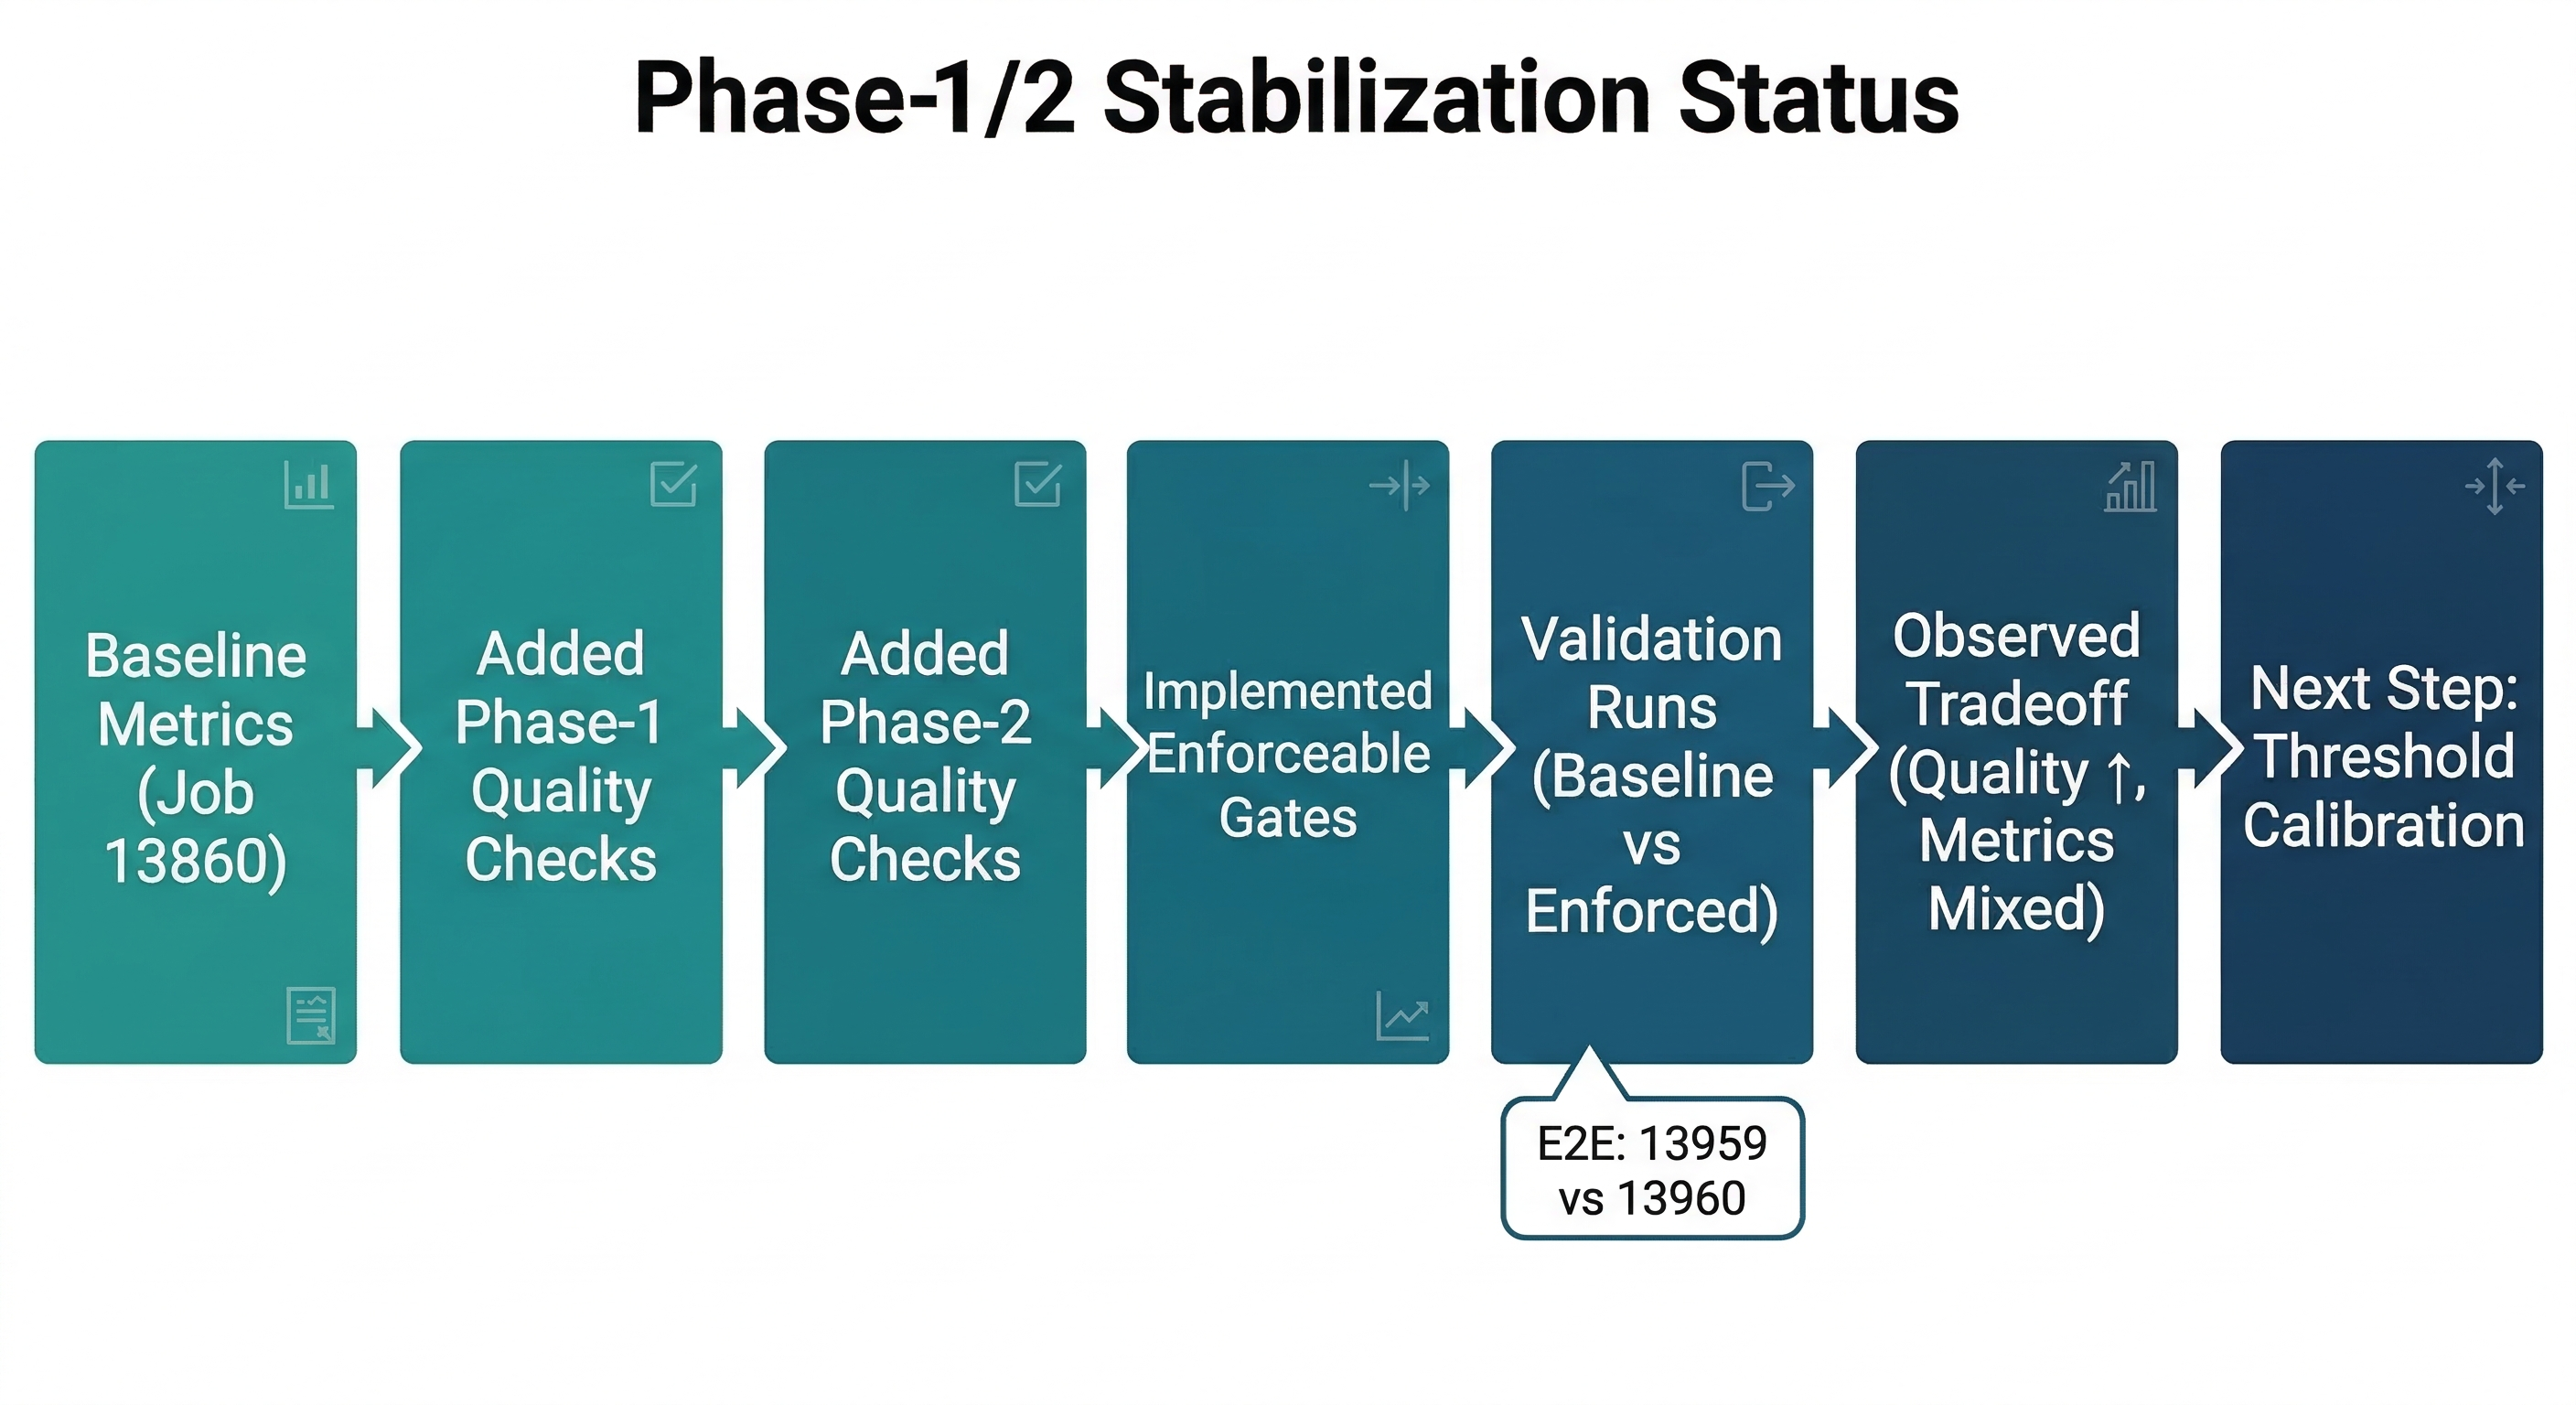
\includegraphics[width=0.95\textwidth]{fig_exec_flow.png}
\caption{Executive flowchart for status meeting discussion.}
\end{figure}

\section{Upnext Tasks (Phase 3, Phase 4, Phase 5)}
\subsection{Phase 3 planned qualitative assessments and changes}
\begin{itemize}[leftmargin=1.2em]
    \item Add class-wise retention diagnostics after filtering (AD/MCI survival curves).
    \item Add plausibility drift checks pre-vs-post filtering (spectral and topology deltas).
    \item Planned change: co-calibrate $\tau_{min},\tau_{max}$ with phase-2 min-keep to prevent minority over-pruning.
\end{itemize}

\subsection{Phase 4 planned qualitative assessments and changes}
\begin{itemize}[leftmargin=1.2em]
    \item Embedding separability checks (class overlap in latent space) for real-vs-synthetic mixes.
    \item Augmentation robustness checks across perturbation strengths.
    \item Planned change: use a compact controlled sweep to avoid confounding while tuning representation stability.
\end{itemize}

\subsection{Phase 5 planned qualitative assessments and changes}
\begin{itemize}[leftmargin=1.2em]
    \item Class-wise calibration and confusion trend tracking by epoch.
    \item Variance tracking across repeated fixed-config runs.
    \item Planned change: jointly tune synthetic caps (AD/MCI) and weight mode to balance AD and MCI recall.
\end{itemize}

\section{Post-Meeting Execution Plan}
\begin{enumerate}[leftmargin=1.2em]
    \item Phase-2/3 co-calibration run pack (small, controlled).
    \item Phase-5 cap/weight re-optimization on calibrated retained sets.
    \item Reproducibility validation with 2--3 fixed-configuration E2E runs.
\end{enumerate}

\end{document}
